\section{Discussion}
\label{sec:discussion}

\subsection{The rank does not transfer across grains}
\label{sec:grain-dependence}

A single ``best model'' would erase the result in Table~\ref{tab:top3}.
The monthly panel is short, strongly seasonal, and paired with a debt-stock covariate.
There a local switch between boosting and the seasonal naive (E2) reduces test sMAPE relative to either piece alone.
The daily and weekly slip aggregates are longer, and the zero-shot foundation model leads them.
TimesFM does not lead the monthly panel: Table~\ref{tab:monthly} places it behind the seasonal naive, with negative skill.
That split is consistent with a pretraining advantage on long, high-frequency series and with a short monthly sample on which a seasonal copy remains hard to beat.
Selective TEM is the only Stage~2 row that estimates an energy and can abstain under~\eqref{eq:tem}.
On the monthly freeze its sMAPE is worse than the seasonal naive, so the energy rule did not pay for itself on that 12-month test.
Where E1 is considered as a monitoring instrument, the relevant extra output is coverage, not a claim that its point sMAPE dominates the ladder.

\begin{figure}[t]
  \centering
  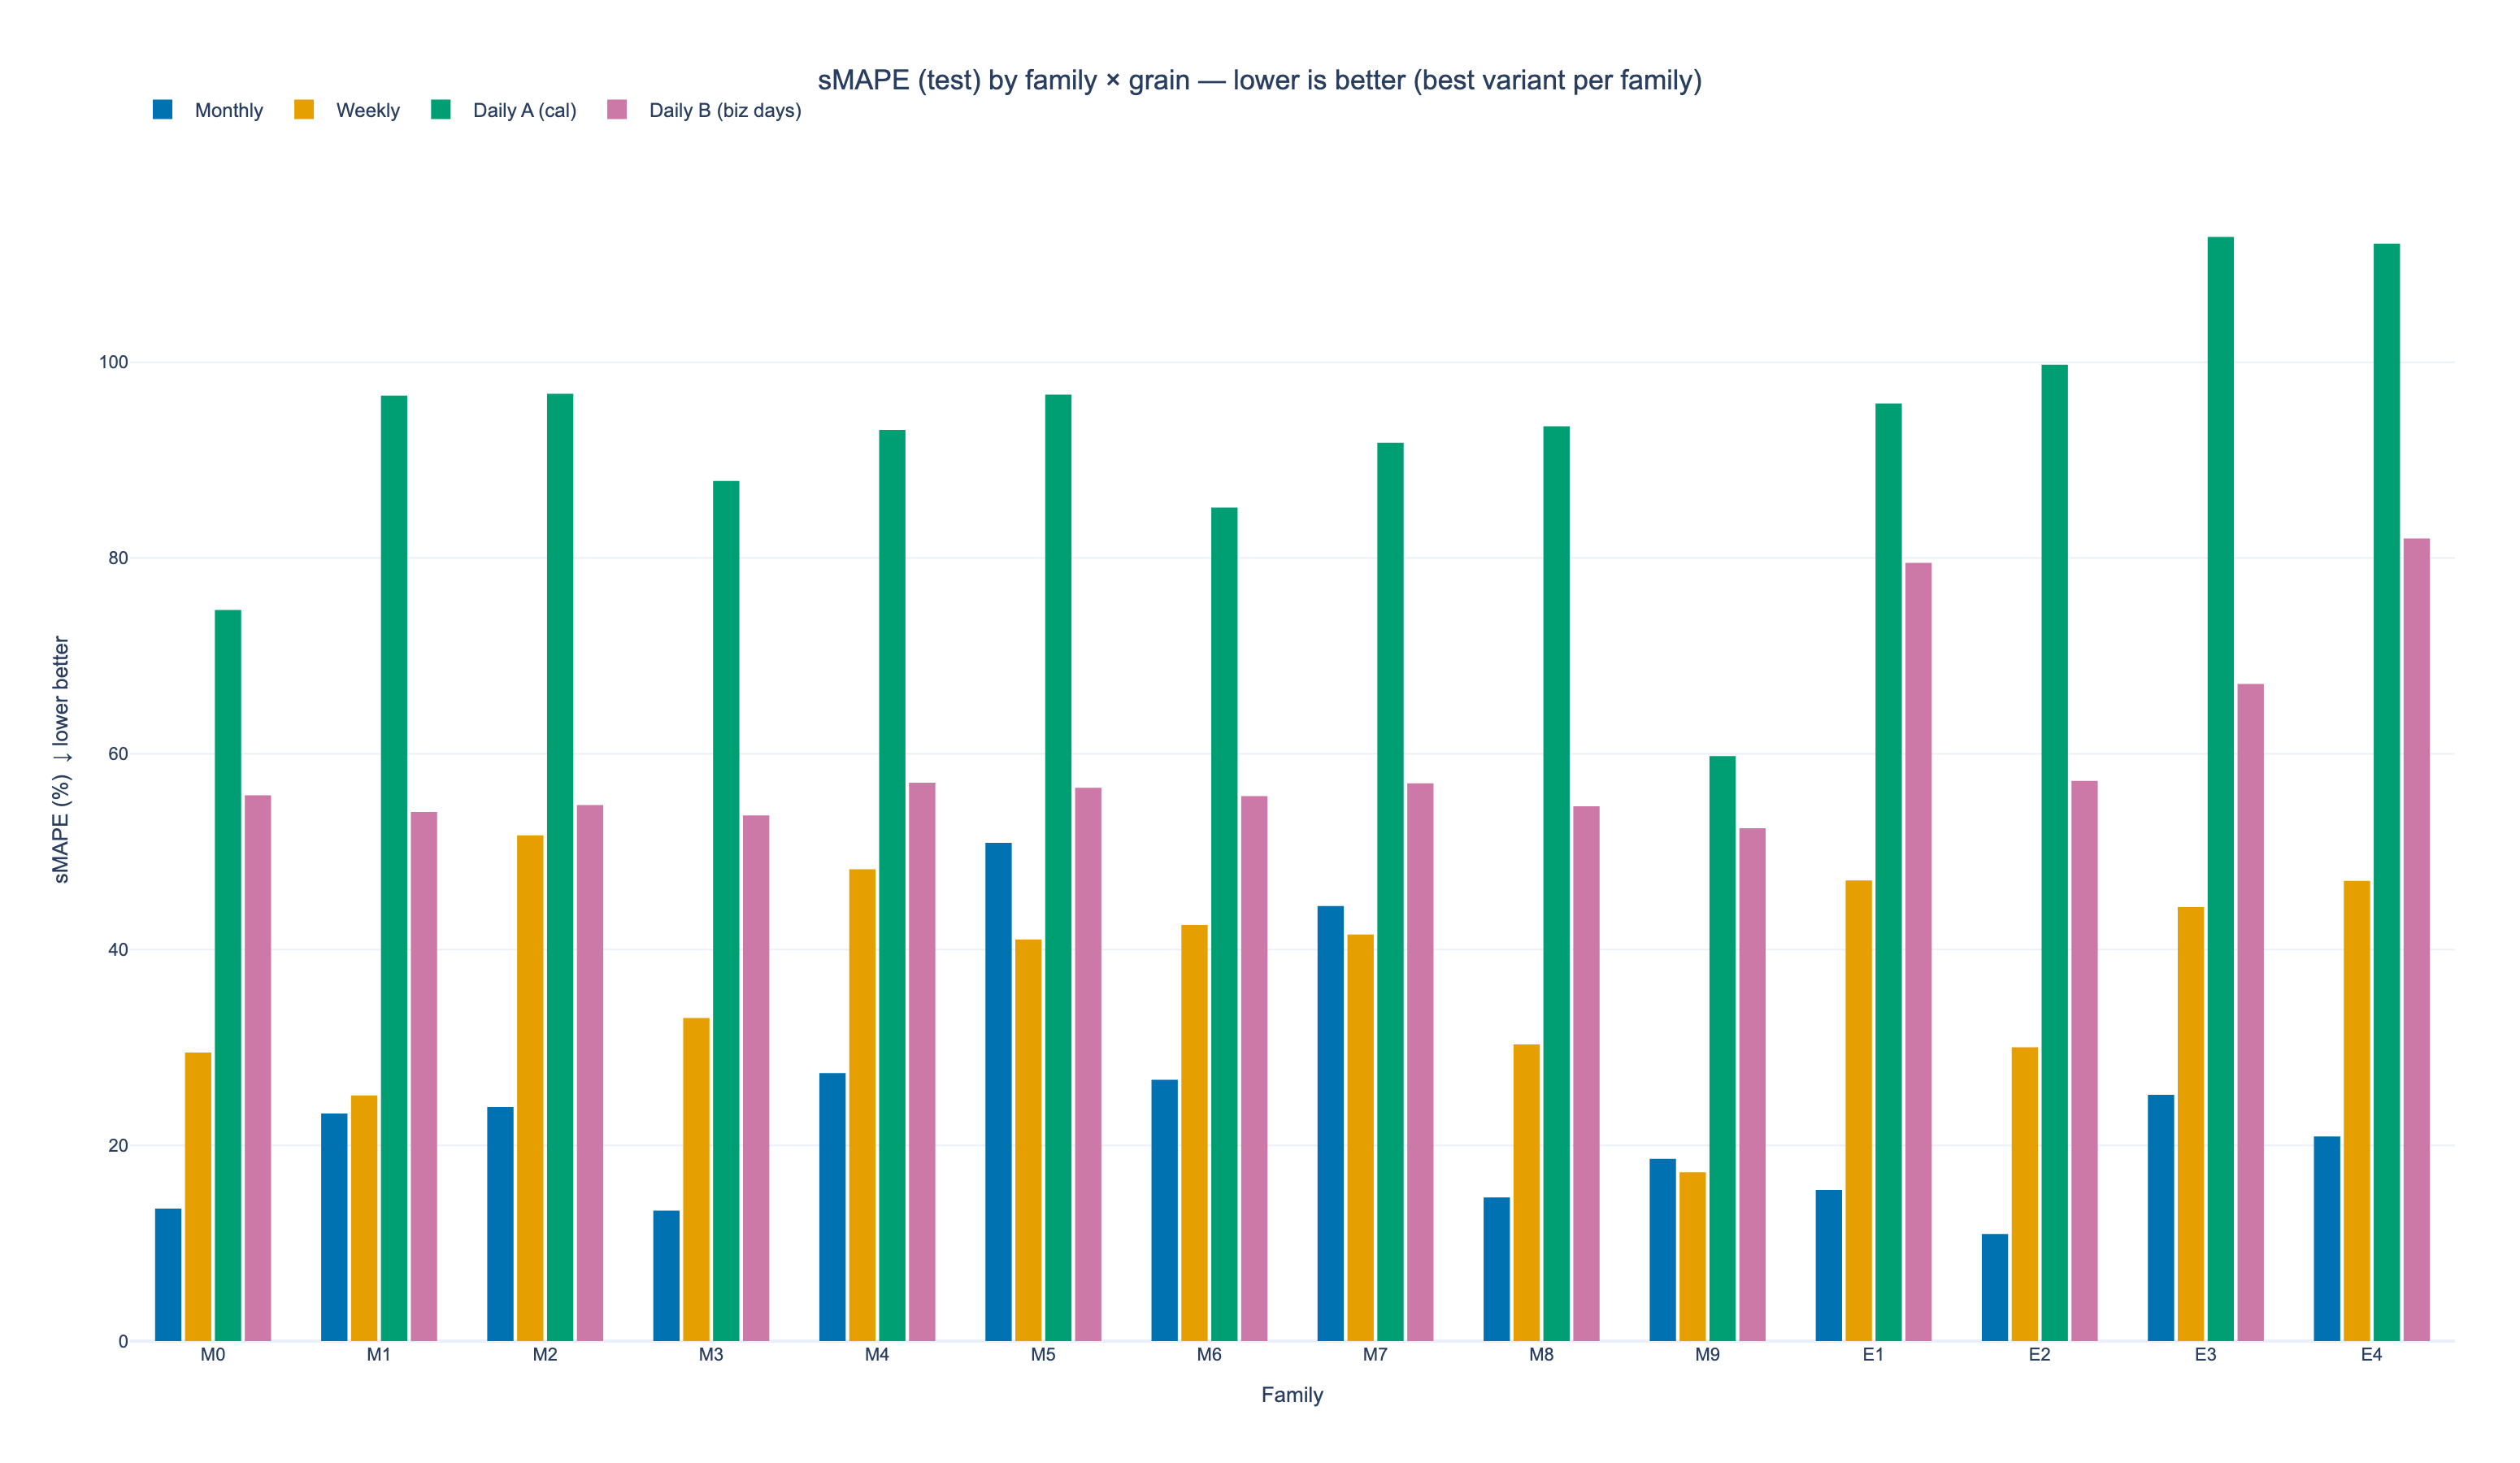
\includegraphics[width=\linewidth]{figures/paper_v1_discussion_compare_smape_by_grain.png}
  \caption{Test sMAPE by model family and grain.
  The vertical axis is the official ranking score (percent, lower is better).
  Families are not averaged across grains.}
  \label{fig:smape_grain}
\end{figure}

\begin{figure}[t]
  \centering
  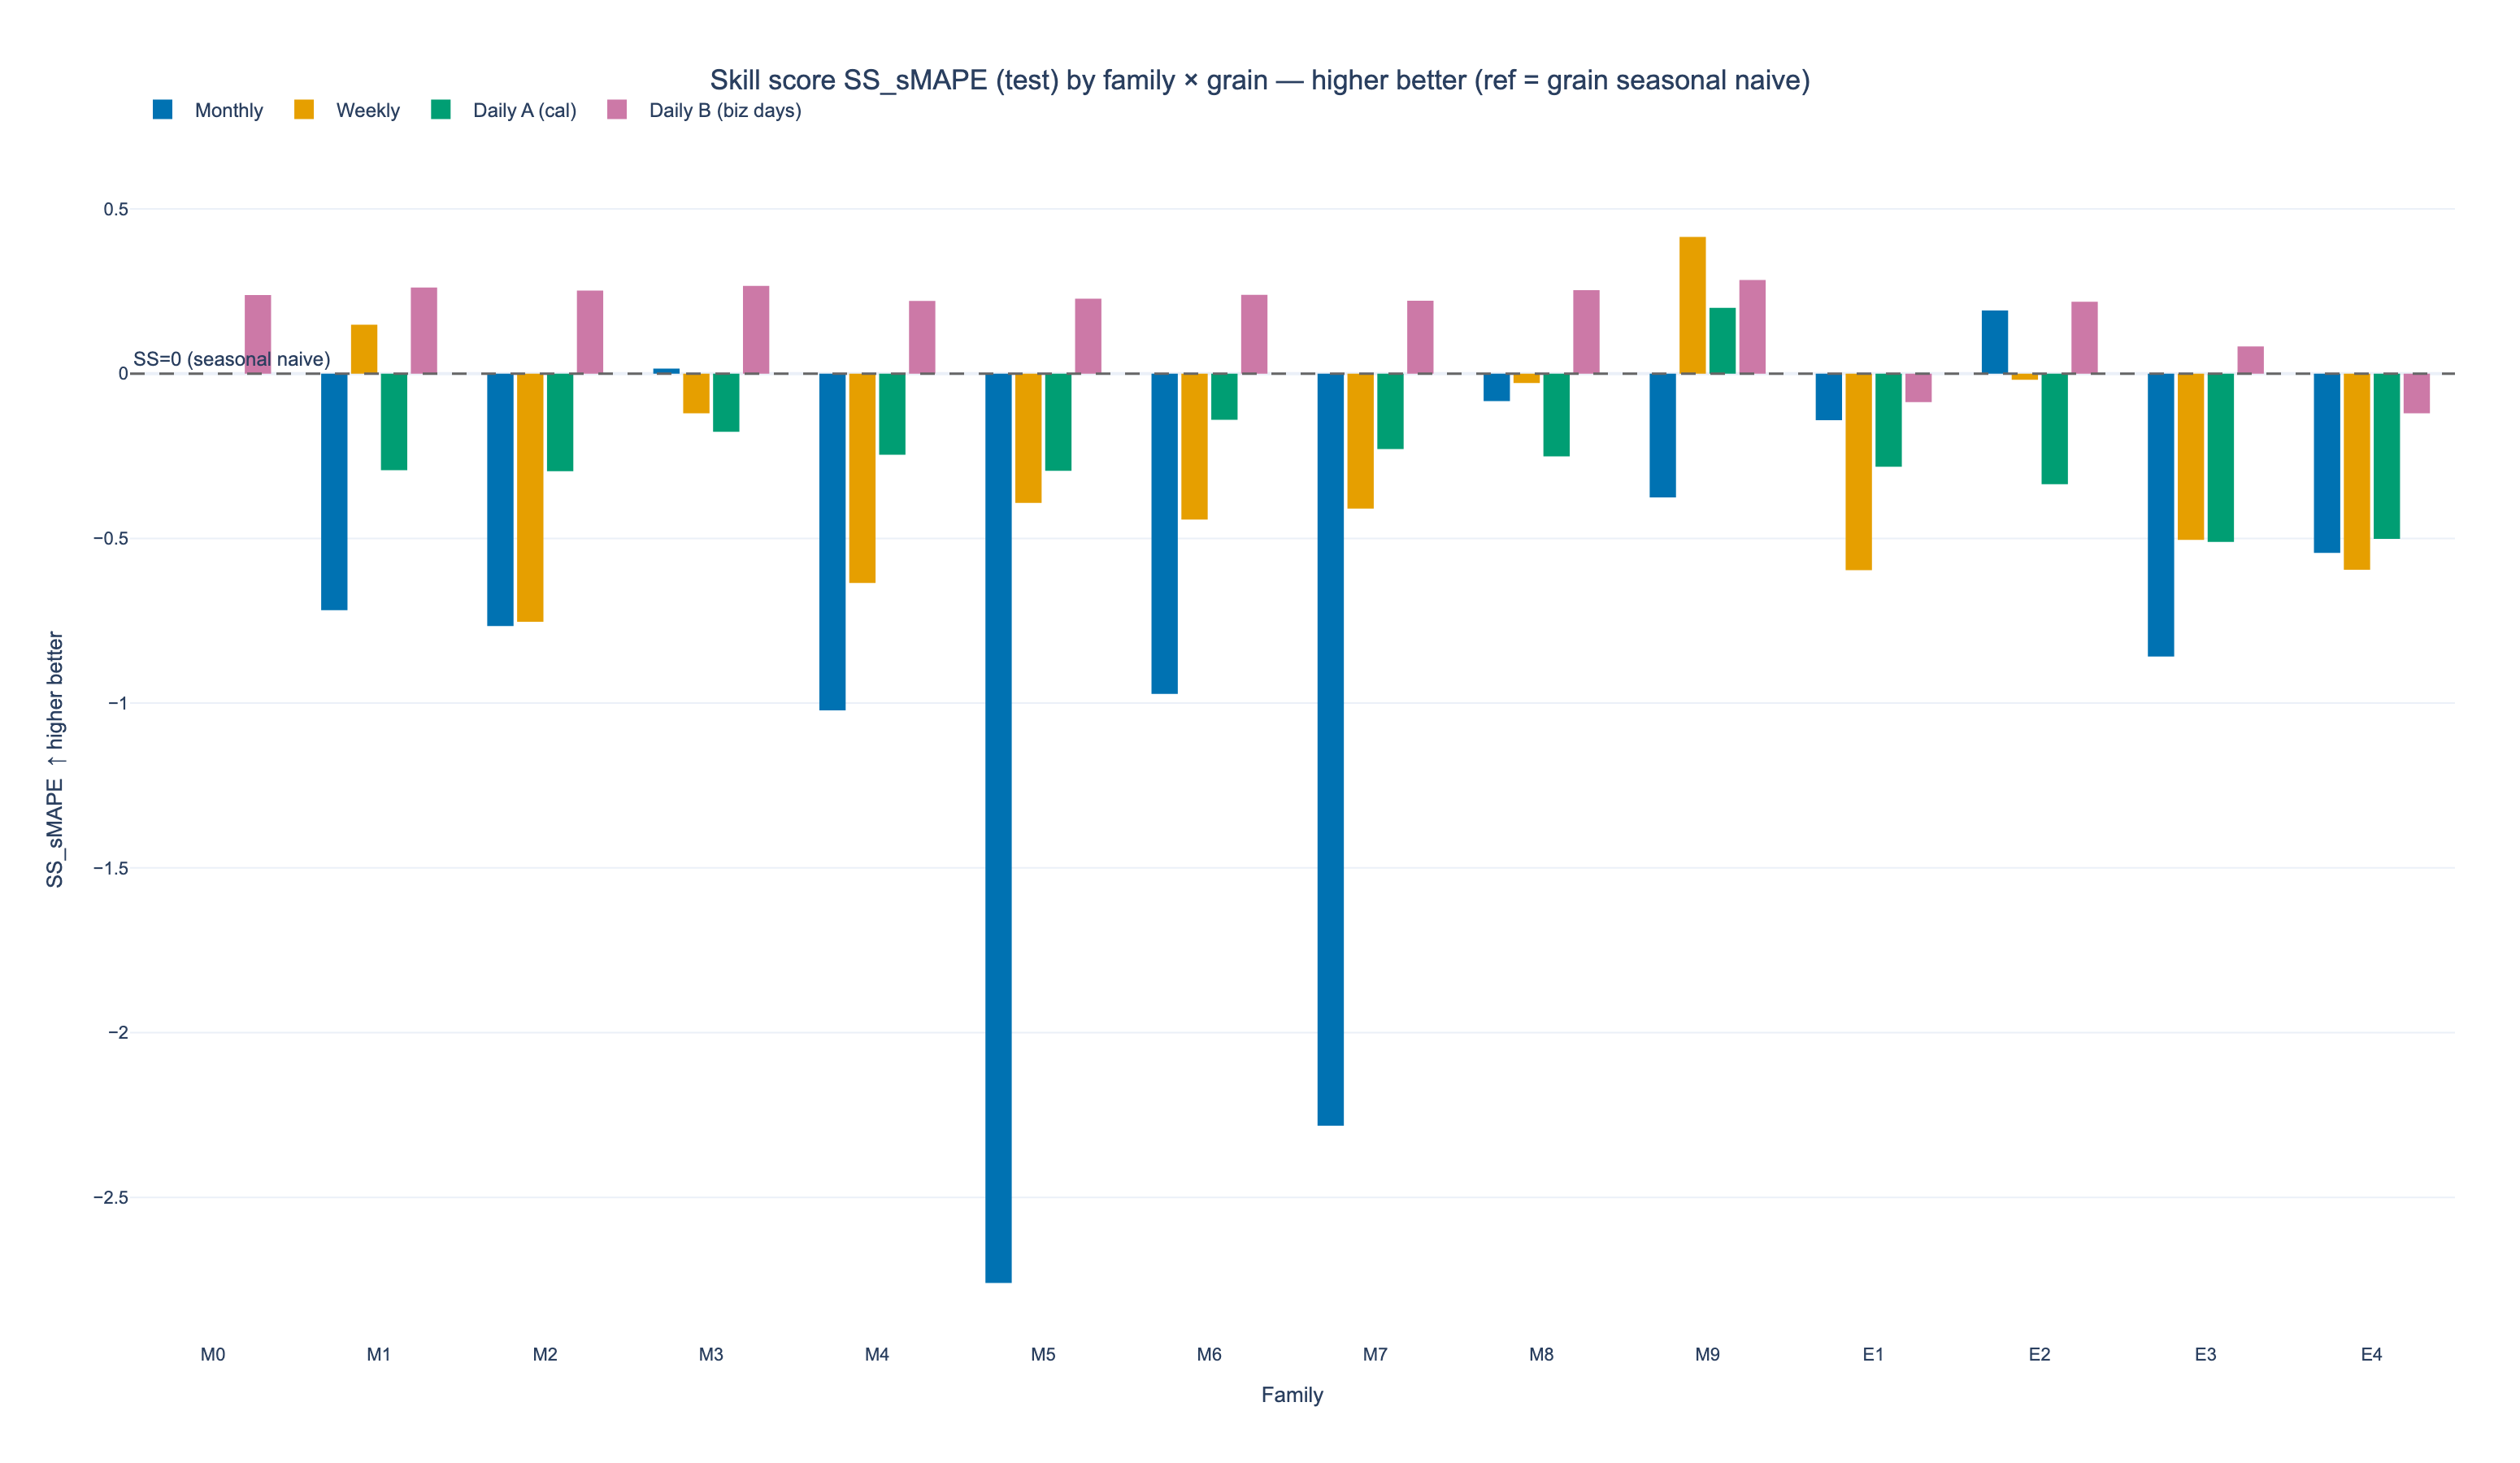
\includegraphics[width=\linewidth]{figures/paper_v1_discussion_compare_skill_by_grain.png}
  \caption{Skill score~\eqref{eq:ss} by model family and grain.
  Zero is the seasonal naive of that grain.
  Positive values beat that naive on sMAPE.
  Negative values do not.}
  \label{fig:ss_grain}
\end{figure}

Figure~\ref{fig:smape_grain} shows the level gap: monthly and weekly sMAPE sit far below calendar-daily sMAPE, because a week or a month aggregates away many structural zeros.
Figure~\ref{fig:ss_grain} shows that this level gap is not the same fact as skill.
A model can post a moderate sMAPE and still lose to a strong seasonal naive, which is the common pattern on the monthly panel, on Ranking~A, and on the weekly series outside TimesFM, ridge, and ordinary least squares.

\subsection{Zeros, holidays, and what the skill score is relative to}
\label{sec:zeros}

On Ranking~A the seasonal naive at lag~7 is second in Table~\ref{tab:ablation}, and most other families have negative skill against it.
Weekend and empty-slip zeros are easy for a weekly copy and difficult for a model that smooths through them.
Restricting the score to $y \gt 0$ lowers sMAPE sharply, as reported in Section~\ref{sec:ablation}, which confirms that the official number is an all-day number.
Using only the positive days as the target would answer a different question: forecast quality on days when a slip was issued, not forecast quality of the calendar a monitoring desk actually sees.

\begin{figure}[t]
  \centering
  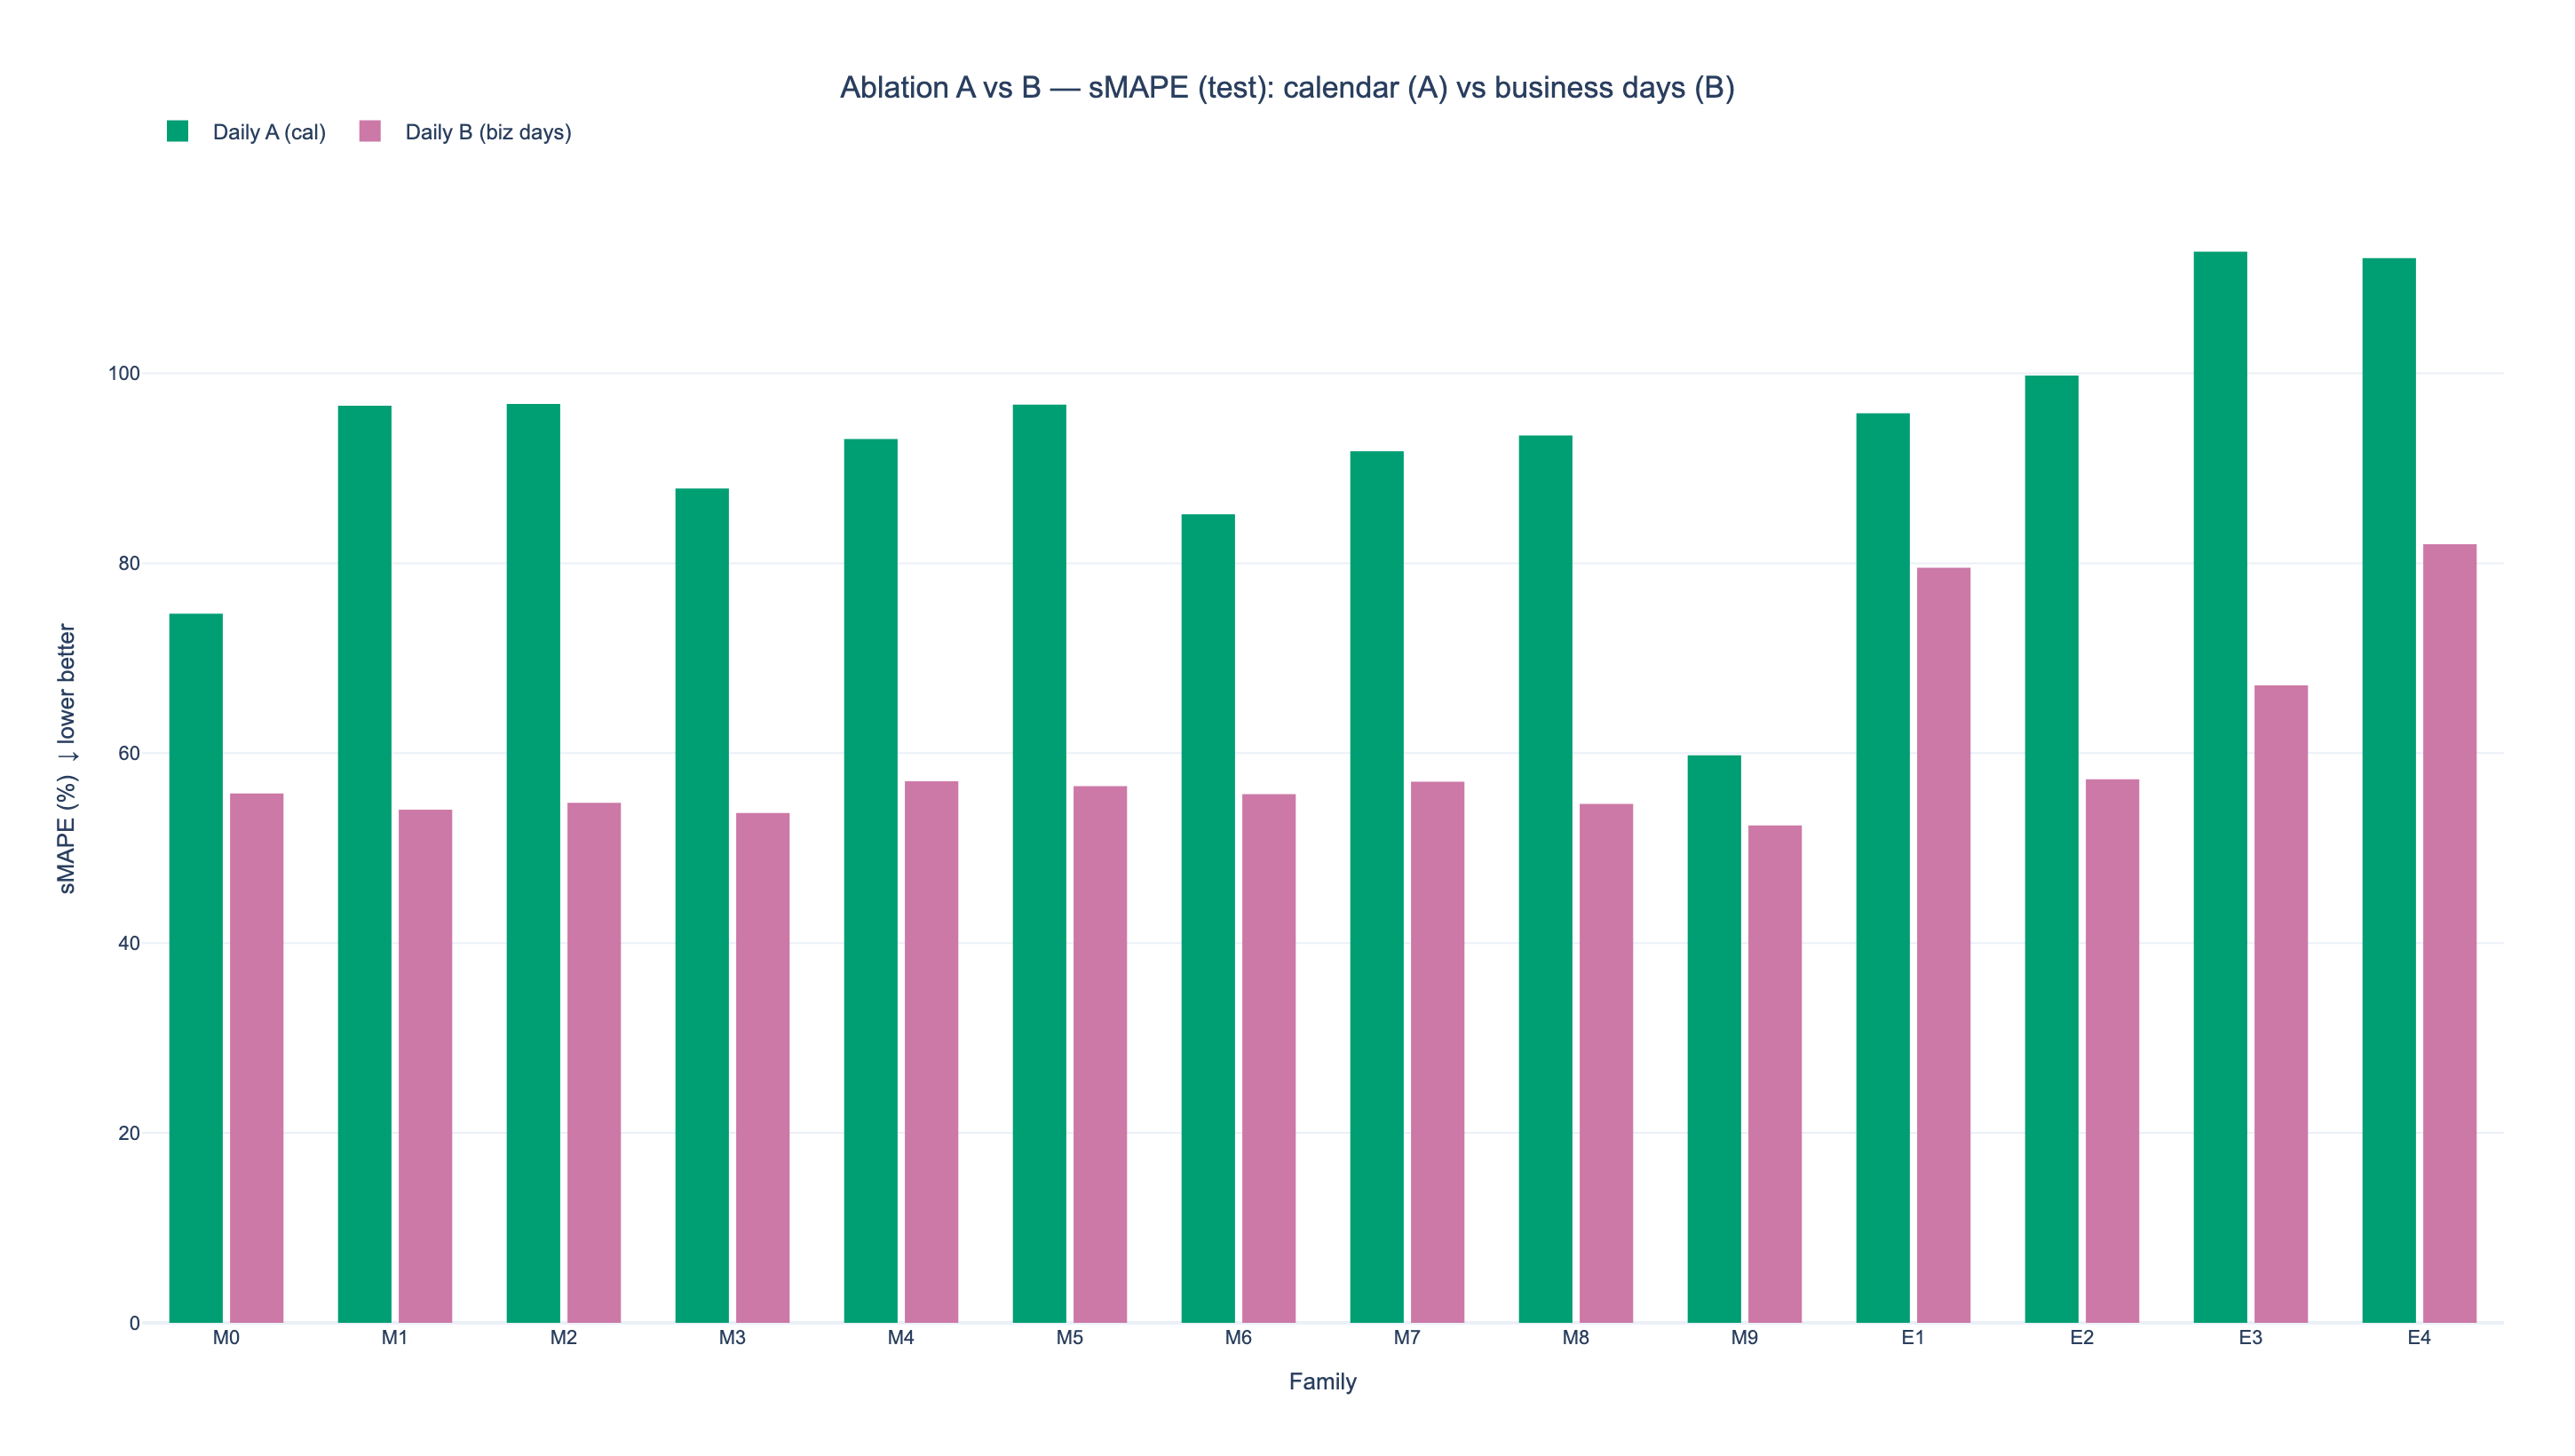
\includegraphics[width=\linewidth]{figures/paper_v1_discussion_compare_ablation_smape.png}
  \caption{Test sMAPE for the calendar-daily series (A) and the business-day series (B).
  B drops weekends and keeps Brazilian national holidays.
  Lower is better.
  The two panels are different targets.}
  \label{fig:abl_smape}
\end{figure}

\begin{figure}[t]
  \centering
  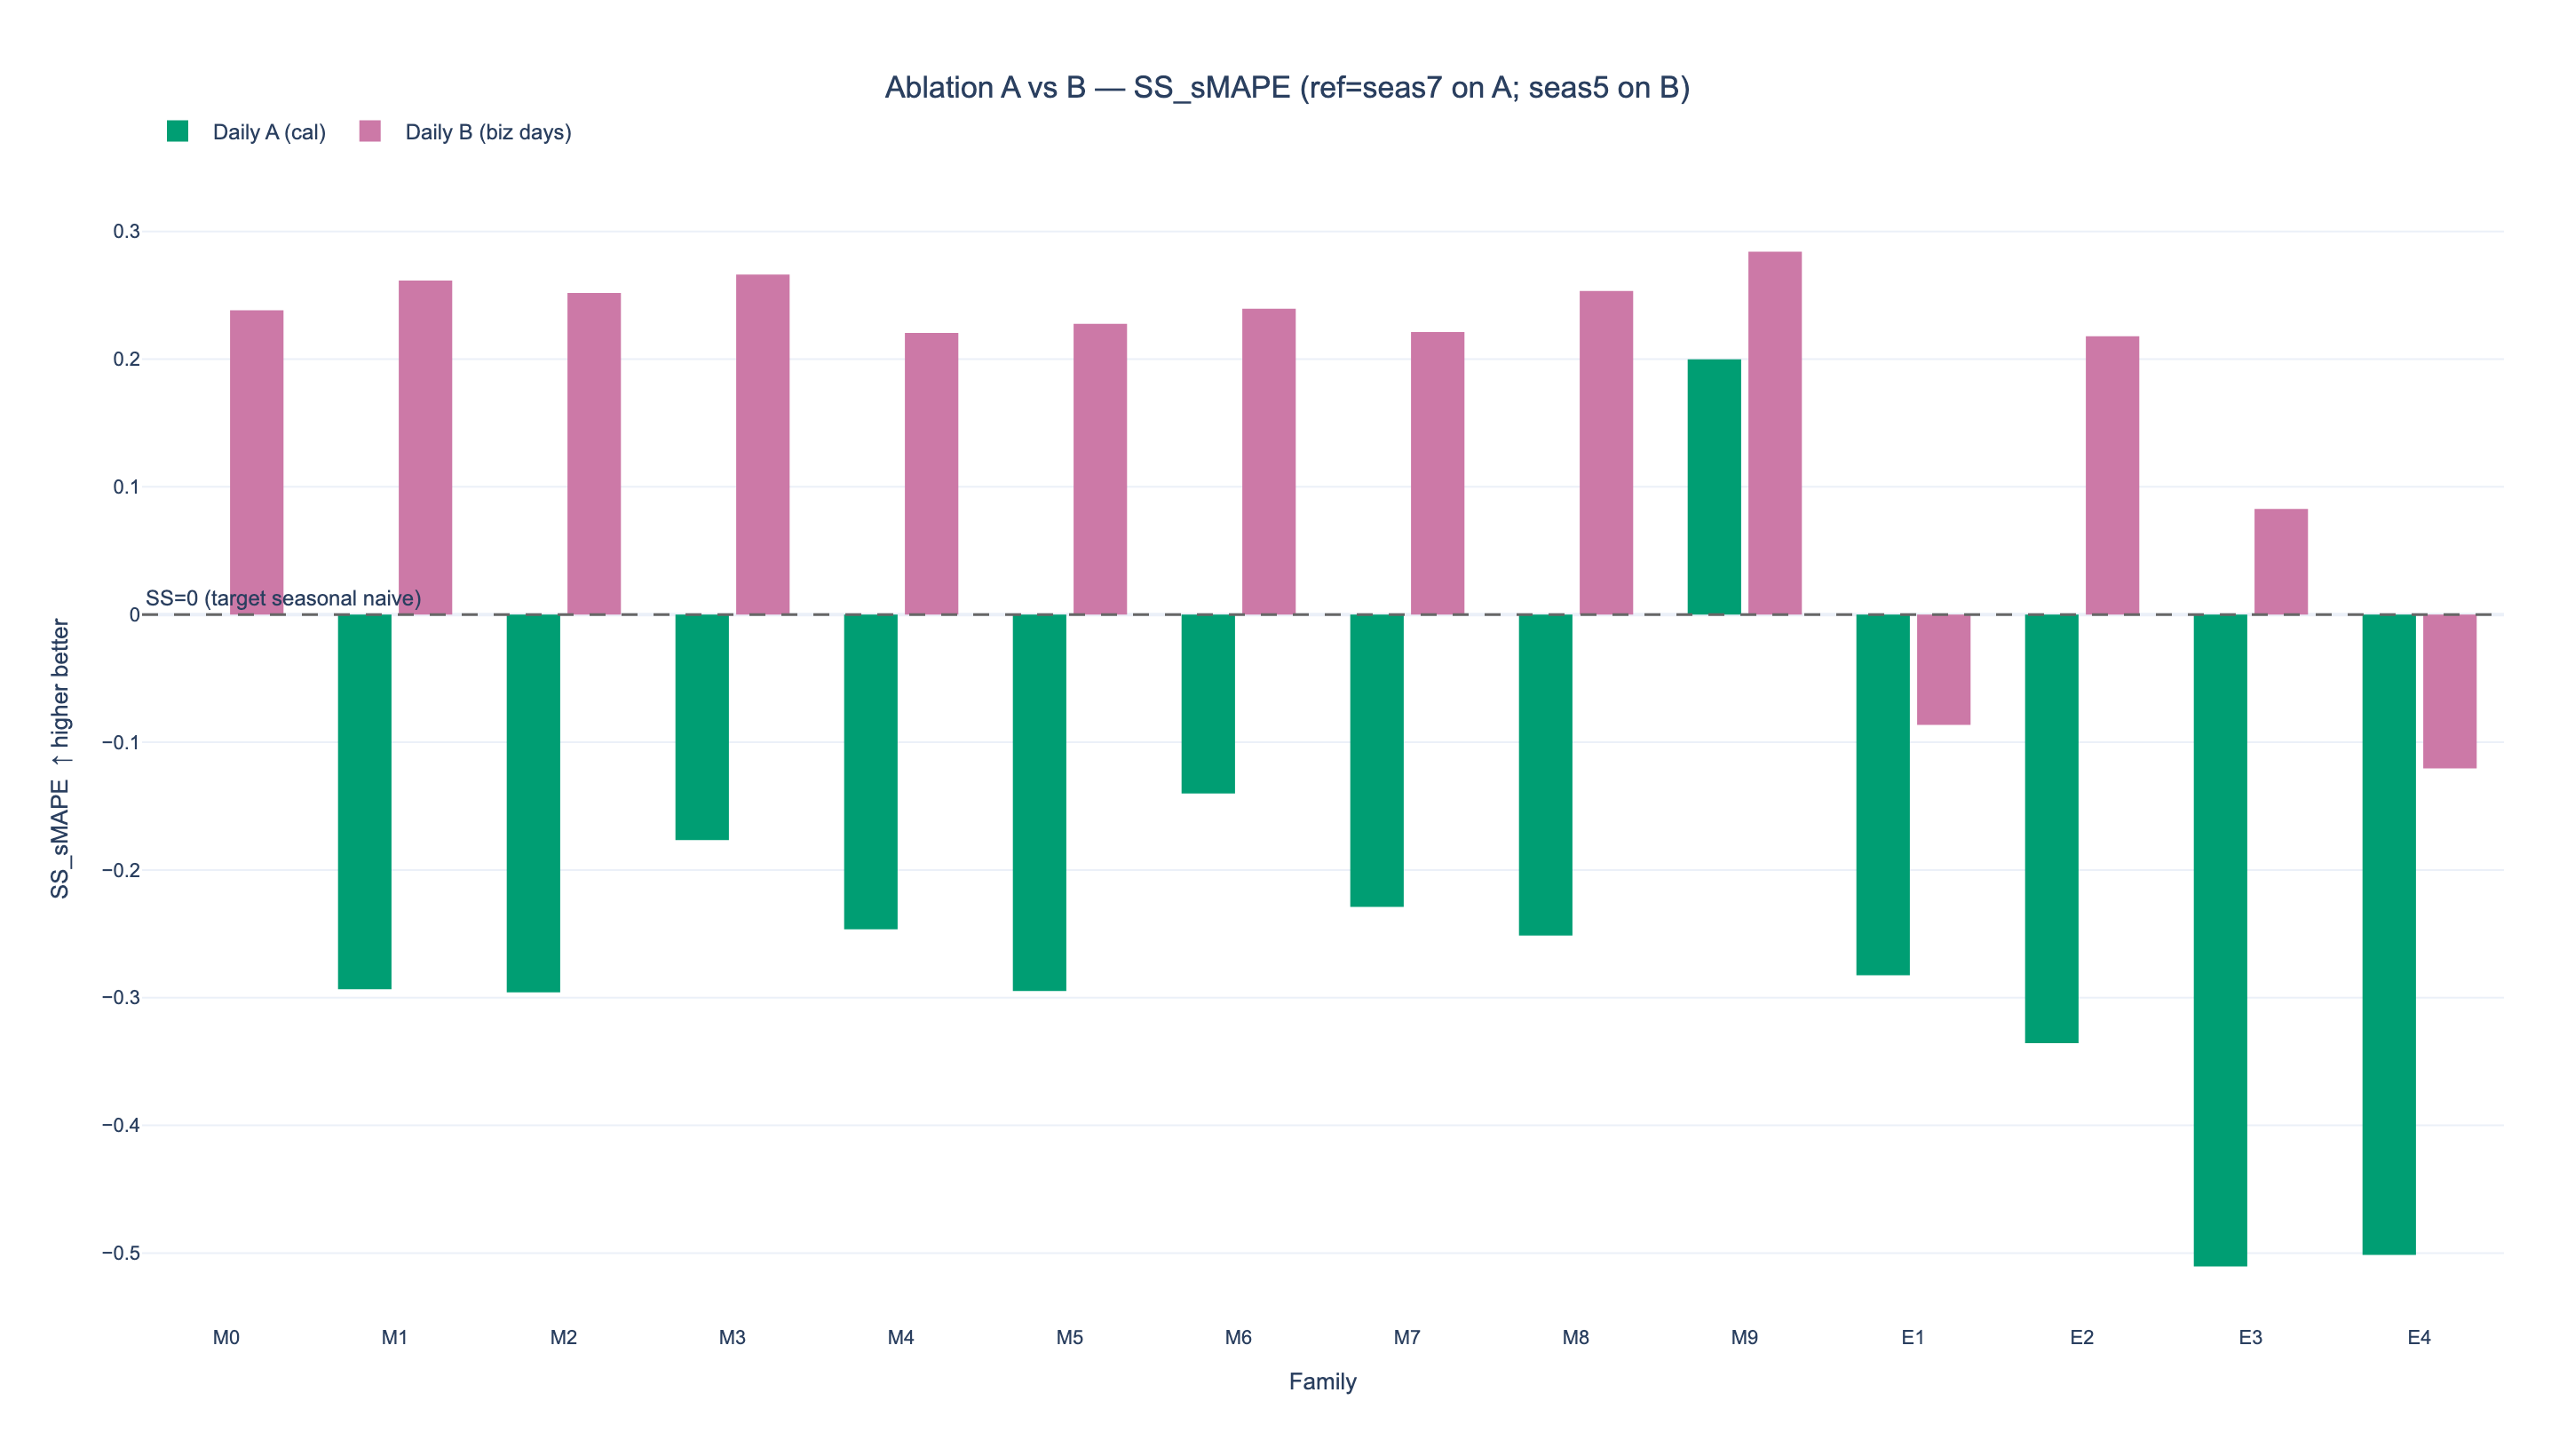
\includegraphics[width=\linewidth]{figures/paper_v1_discussion_compare_ablation_skill.png}
  \caption{Skill score against the seasonal naive of each daily target: lag~7 on A and lag~5 on B.
  Positive skill on B is skill against lag~5, which is a weak reference on this series.}
  \label{fig:abl_ss}
\end{figure}

Ranking~B removes weekends and leaves national holidays in the series (Figure~\ref{fig:abl_smape}).
Absolute sMAPE falls, and boosting and ordinary least squares enter the top three beside TimesFM.
Skill on B is measured against lag~5 (Figure~\ref{fig:abl_ss}).
Many positive scores appear because that reference is weak: the lag-1 naive already beats it.
Those scores do not say that the same models beat a lag-1 forecast, and they do not transfer to Ranking~A, whose reference is lag~7.
Holiday effects that fall on weekdays remain inside both the series and the residual of every model that was not given a holiday calendar.
Prophet was not given one.

\subsection{What can serve as a monitoring instrument}
\label{sec:instrument}

The seasonal naive is the reference instrument.
It costs nothing to compute, it scores zero skill by construction, and on several grains it remains inside the top three on sMAPE.
Any replacement has to beat it on the grain that will be published.

E1 is the selective candidate.
Equation~\eqref{eq:tem} returns either a minimum-energy candidate or the seasonal naive, which is the right shape for a desk that would rather abstain than publish a low-confidence number.
The monthly freeze does not show an sMAPE gain for that rule.
Until coverage is reported beside sMAPE, E1 should be read as a specified decision rule, not as the operational default.

E2's monthly lead is real on this freeze and easy to over-read.
The rule in~\eqref{eq:proxy-rule} is a validation-chosen switch between two Stage~1 forecasts.
It demonstrates that disagreement with the seasonal naive is an informative abstention signal on the monthly panel.
It does not estimate~\eqref{eq:ebm}, it was not trained as TEM, and a gain for E2 is not a gain for E1.

TimesFM is the operational lead on both daily rankings and on the weekly aggregate in this freeze, under a zero-shot protocol.
Figure~\ref{fig:pred} overlays realized collection with the holdout paths of the highest-ranked forecasts on each grain.
On the monthly panel that set includes the disagreement proxy, which is the sMAPE leader, and it does not identify that path with selective TEM.
On the daily and weekly panels the set includes TimesFM~3.0.
The practical caveat is dependence on an external checkpoint and on a context window that, on the monthly panel, was not long enough for that checkpoint to beat the seasonal naive.
A monitoring deployment that needs a number when the checkpoint is unavailable still has the seasonal naive, and on the monthly grain that fallback is competitive.

\begin{figure}[t]
  \centering
  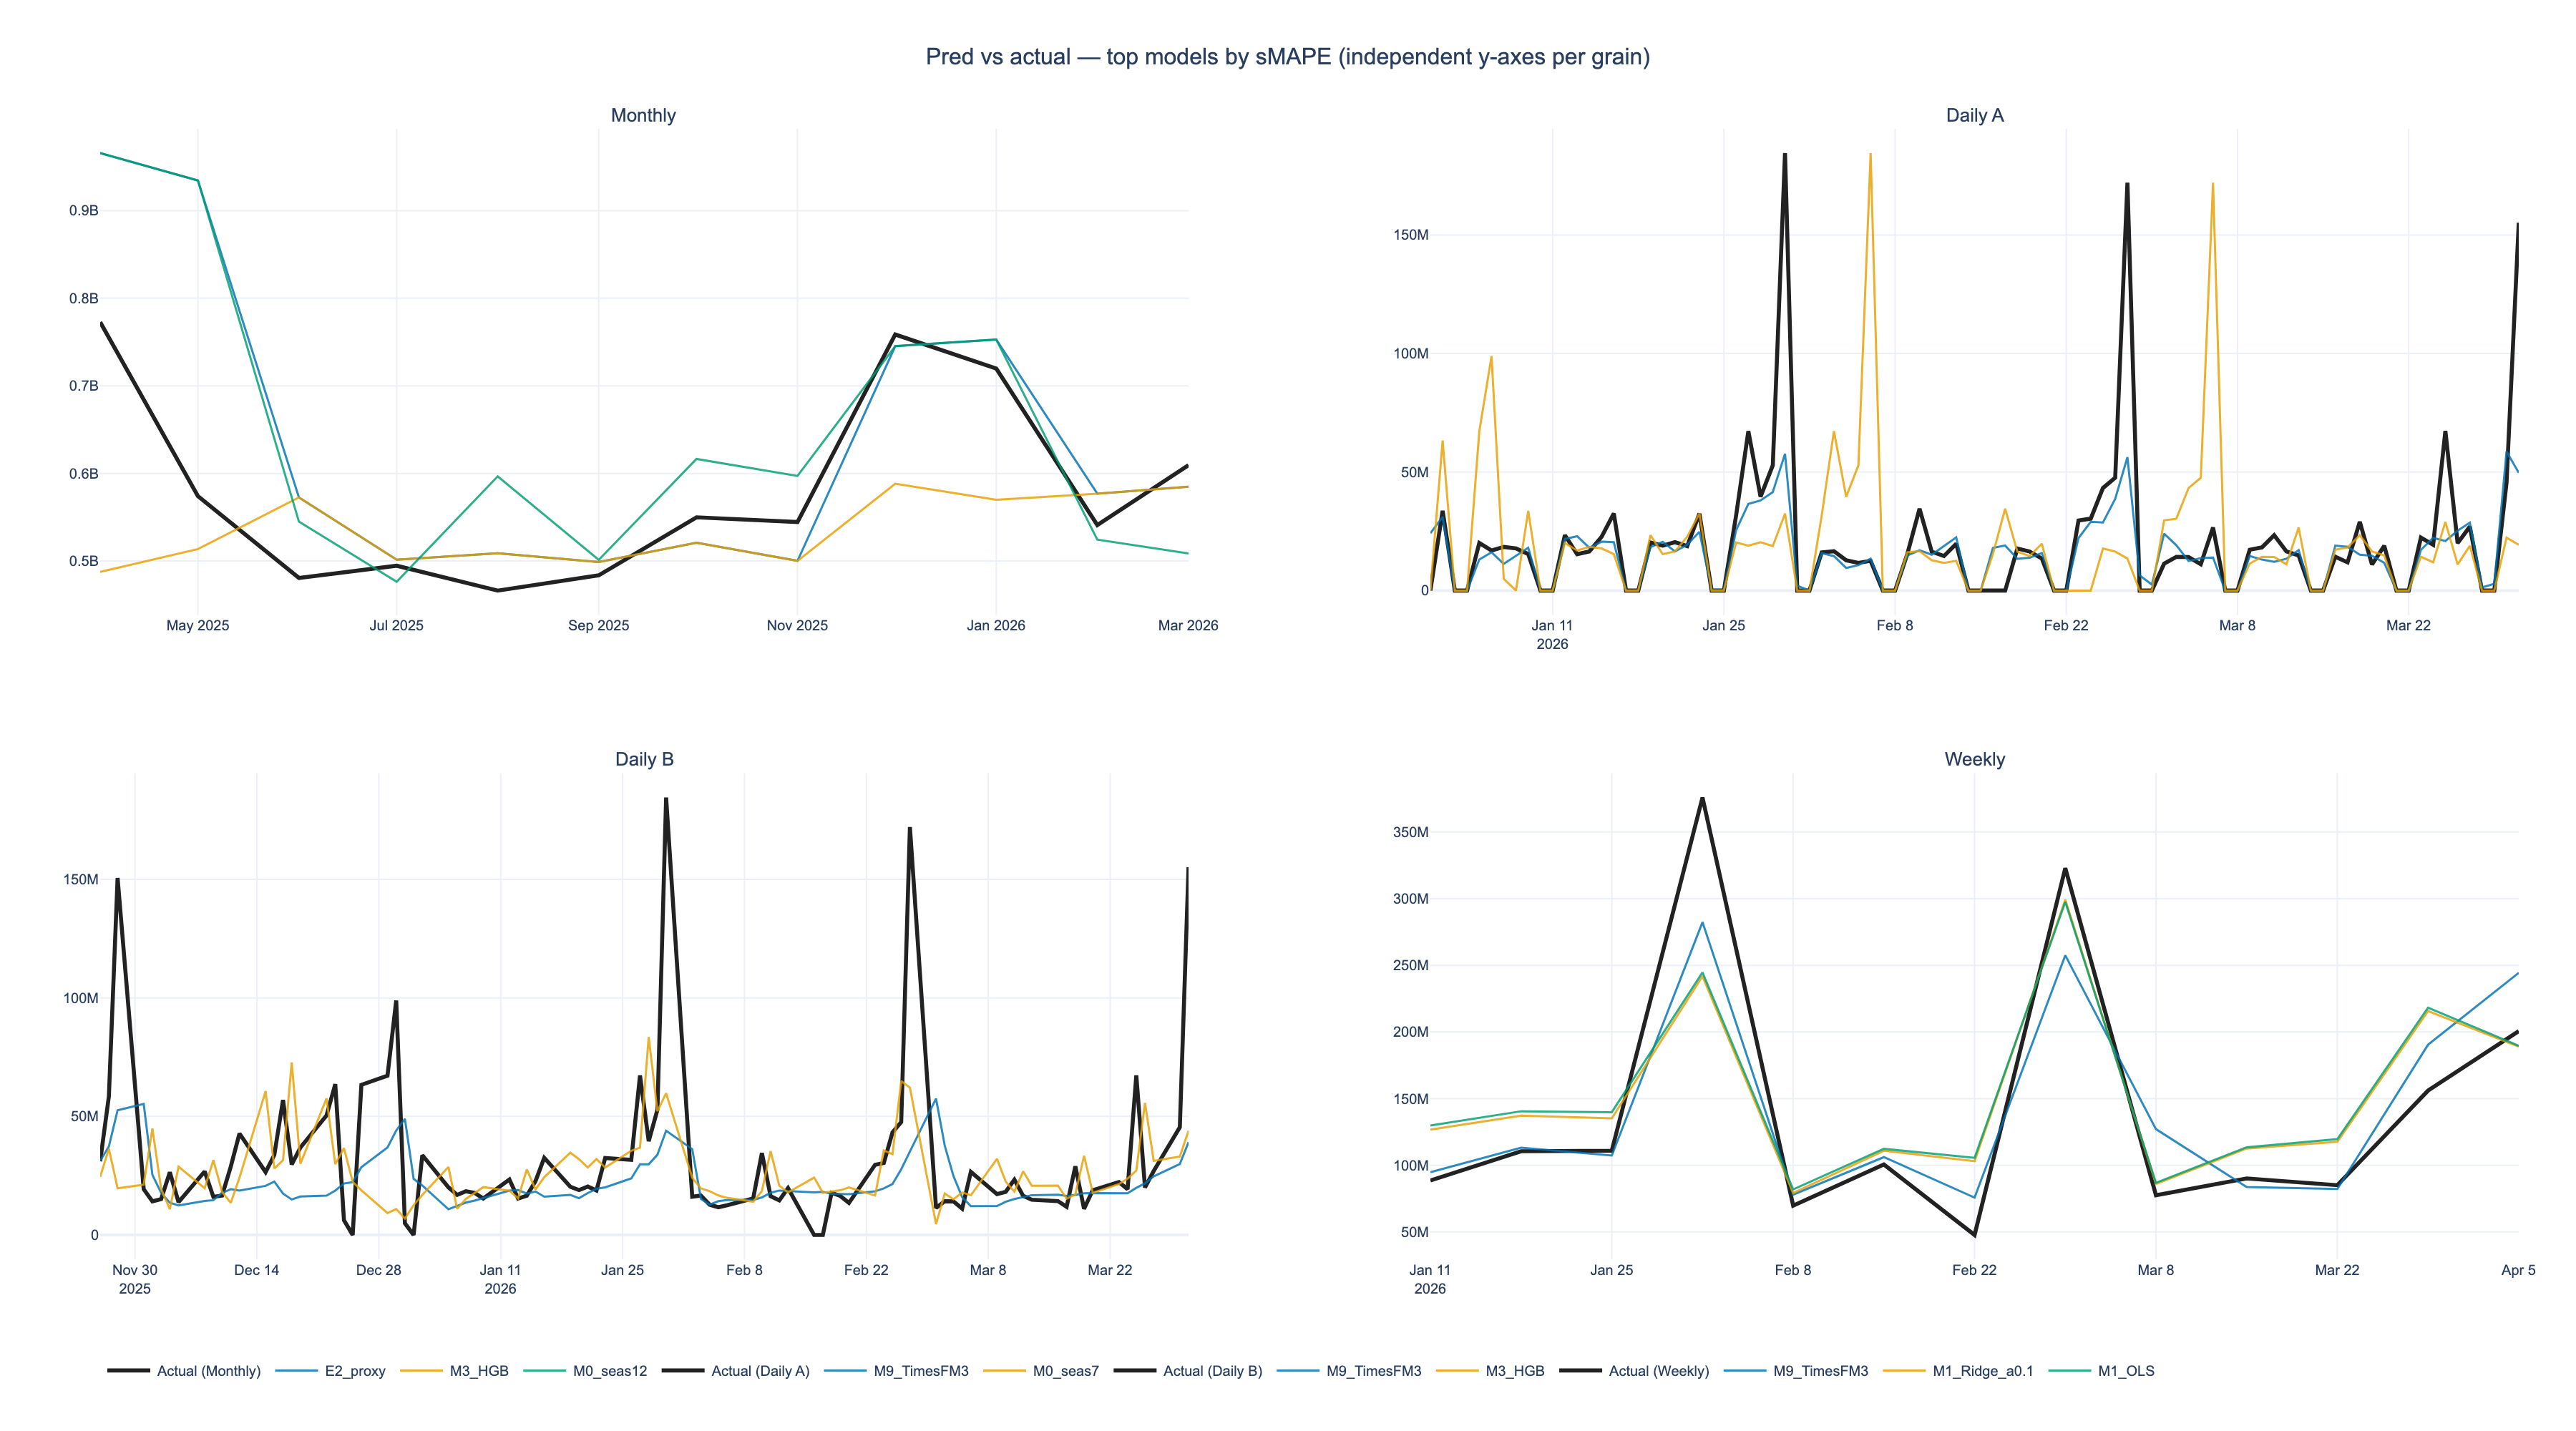
\includegraphics[width=\linewidth]{figures/paper_v1_discussion_pred_vs_actual_top.png}
  \caption{Holdout paths of realized collection and of the highest-ranked point forecasts on each grain.
  The monthly panel's sMAPE leader in this comparison is the disagreement proxy.
  The daily and weekly leaders are TimesFM~3.0.
  Selective TEM is a separate row and is not that monthly leader.}
  \label{fig:pred}
\end{figure}
